% Options for packages loaded elsewhere
\PassOptionsToPackage{unicode}{hyperref}
\PassOptionsToPackage{hyphens}{url}
%
\documentclass[
]{book}
\usepackage{amsmath,amssymb}
\usepackage{iftex}
\ifPDFTeX
  \usepackage[T1]{fontenc}
  \usepackage[utf8]{inputenc}
  \usepackage{textcomp} % provide euro and other symbols
\else % if luatex or xetex
  \usepackage{unicode-math} % this also loads fontspec
  \defaultfontfeatures{Scale=MatchLowercase}
  \defaultfontfeatures[\rmfamily]{Ligatures=TeX,Scale=1}
\fi
\usepackage{lmodern}
\ifPDFTeX\else
  % xetex/luatex font selection
\fi
% Use upquote if available, for straight quotes in verbatim environments
\IfFileExists{upquote.sty}{\usepackage{upquote}}{}
\IfFileExists{microtype.sty}{% use microtype if available
  \usepackage[]{microtype}
  \UseMicrotypeSet[protrusion]{basicmath} % disable protrusion for tt fonts
}{}
\makeatletter
\@ifundefined{KOMAClassName}{% if non-KOMA class
  \IfFileExists{parskip.sty}{%
    \usepackage{parskip}
  }{% else
    \setlength{\parindent}{0pt}
    \setlength{\parskip}{6pt plus 2pt minus 1pt}}
}{% if KOMA class
  \KOMAoptions{parskip=half}}
\makeatother
\usepackage{xcolor}
\usepackage{longtable,booktabs,array}
\usepackage{calc} % for calculating minipage widths
% Correct order of tables after \paragraph or \subparagraph
\usepackage{etoolbox}
\makeatletter
\patchcmd\longtable{\par}{\if@noskipsec\mbox{}\fi\par}{}{}
\makeatother
% Allow footnotes in longtable head/foot
\IfFileExists{footnotehyper.sty}{\usepackage{footnotehyper}}{\usepackage{footnote}}
\makesavenoteenv{longtable}
\usepackage{graphicx}
\makeatletter
\def\maxwidth{\ifdim\Gin@nat@width>\linewidth\linewidth\else\Gin@nat@width\fi}
\def\maxheight{\ifdim\Gin@nat@height>\textheight\textheight\else\Gin@nat@height\fi}
\makeatother
% Scale images if necessary, so that they will not overflow the page
% margins by default, and it is still possible to overwrite the defaults
% using explicit options in \includegraphics[width, height, ...]{}
\setkeys{Gin}{width=\maxwidth,height=\maxheight,keepaspectratio}
% Set default figure placement to htbp
\makeatletter
\def\fps@figure{htbp}
\makeatother
\setlength{\emergencystretch}{3em} % prevent overfull lines
\providecommand{\tightlist}{%
  \setlength{\itemsep}{0pt}\setlength{\parskip}{0pt}}
\setcounter{secnumdepth}{5}
\usepackage{booktabs}
\ifLuaTeX
  \usepackage{selnolig}  % disable illegal ligatures
\fi
\usepackage[]{natbib}
\bibliographystyle{plainnat}
\usepackage{bookmark}
\IfFileExists{xurl.sty}{\usepackage{xurl}}{} % add URL line breaks if available
\urlstyle{same}
\hypersetup{
  pdftitle={ADS - Tecnologia da Informação e Telecomunicações 2025 - Anotações de aula},
  pdfauthor={Professor Miguel Suez Xve Penteado},
  hidelinks,
  pdfcreator={LaTeX via pandoc}}

\title{ADS - Tecnologia da Informação e Telecomunicações 2025 - Anotações de aula}
\author{Professor Miguel Suez Xve Penteado}
\date{2025-02-19}

\begin{document}
\maketitle

{
\setcounter{tocdepth}{1}
\tableofcontents
}
\chapter*{Sobre estas anotações}\label{sobre-estas-anotauxe7uxf5es}
\addcontentsline{toc}{chapter}{Sobre estas anotações}

Estas anotações são apenas lembretes das aulas expostas em sala, durante a disciplina de ENGENHARIA DE SOFTWARE.

\section{ACESSO AO GITBOOK CELULAR}\label{acesso-ao-gitbook-celular}

\section{APP EPUB ANDROID}\label{app-epub-android}

\section{\texorpdfstring{\textbf{Moon+ Reader}}{Moon+ Reader}}\label{moon-reader}

\chapter*{INTRODUÇÃO DA DISCIPLINA}\label{introduuxe7uxe3o-da-disciplina}
\addcontentsline{toc}{chapter}{INTRODUÇÃO DA DISCIPLINA}

coming soon

\section{Livros-Texto da disciplina}\label{livros-texto-da-disciplina}

\subsection{Bibliografia Básica}\label{bibliografia-buxe1sica}

JOÃO, Belmiro N. Informática Aplicada. São Paulo: Pearson Education do Brasil, 2019.

GONÇALVES, G. R. B. Sistemas de informação. Porto Alegre: SAGAH, 2017.

SILVA, K. C. N.; BARBOSA, C.; CÓRDOVA JUNIOR, R. S. Sistemas de informações gerenciais. Porto Alegre: SAGAH, 2018.

\subsection{Bibliografia Complementar}\label{bibliografia-complementar}

LAUDON, Kenneth C; LAUDON, Jane P. Sistemas de Informação Gerenciais. São Paulo: Pearson Education do Brasil, 2014.

MUNHOZ, Antônio S. Fundamentos de Tecnologia da Informação e análise de sistemas para não analistas. Curitiba: Intersaberes, 2017.

MARÇULA, M.; BENINI FILHO, P. A. Informática: Conceitos e Aplicações. 5.Ed. São Paulo: Erica: 2019.

RAINER JUNIOR, R. K.; CEGIELSKI, C. G. Introdução a sistemas de informação. - 5. ed.~- Rio de Janeiro: Elsevier, 2016.

STAIR, Ralph M; REYNOLDS, George W. Princípios de sistemas de informação / Ralph M. Stair. São Paulo: Cengage Learning, 2015.

\chapter{INTRODUÇÃO A TIC (TECNOLOGIA DA INFORMAÇÃO E COMUNICAÇÕES)}\label{introduuxe7uxe3o-a-tic-tecnologia-da-informauxe7uxe3o-e-comunicauxe7uxf5es}

\section{Conceitos de Sistemas de Informação}\label{conceitos-de-sistemas-de-informauxe7uxe3o}

\subsubsection{\texorpdfstring{Conceito de Informação segundo \emph{Kenneth C. LAUDON, Jane P. LAUDON} (2011)}{Conceito de Informação segundo Kenneth C. LAUDON, Jane P. LAUDON (2011)}}\label{conceito-de-informauxe7uxe3o-segundo-kenneth-c.-laudon-jane-p.-laudon-2011}

\begin{figure}
\centering
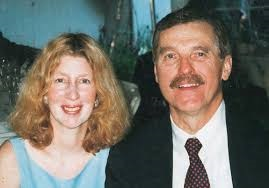
\includegraphics{images/Ken_Jane.jpg}
\caption{Prof Ken C. Laudon (1944 - 2019) e Jane Price Laudon - Universidade Columbia}
\end{figure}

\begin{quote}
\emph{``Tecnicamente, um \textbf{sistema de informação (Si)} é um CONJUNTO DE COMPONENTES RELACIONADOS entre si que COLETAM (ou recuperam), PROCESSAM, ARMAZENAM c DISTRIBUEM {[}o que ?{]} INFORMAÇÕES que servem para apoiar a TOMADA DE DECISÕES, a COORDENAÇÃO e o CONTROLE de uma organização.'' (LAUDON; LAUDON, 2011)}
\end{quote}

PERGUNTA: \emph{Um \textbf{SISTEMA DE INFORMAÇÃO (SI)} é a mesma coisa que um \textbf{computador (smartphone) com um software (app)}}?

a ) sim ? Porque ?\_\_\_\_\_\_\_\_\_\_\_\_\_\_\_\_\_\_\_\_\_\_\_\_\_\_\_\_\_\_\_\_\_\_\_\_\_\_\_\_\_\_\_\_\_\_\_\_\_\_\_\_\_\_\_\_\_\_\_\_\_\_\_\_\_\_\_\_\_\_\_\_\_\_\_\_\_\_\_\_\_\_\_\_\_\_\_\_\_

\begin{enumerate}
\def\labelenumi{\alph{enumi})}
\setcounter{enumi}{1}
\tightlist
\item
  nâo ? Porque ?\_\_\_\_\_\_\_\_\_\_\_\_\_\_\_\_\_\_\_\_\_\_\_\_\_\_\_\_\_\_\_\_\_\_\_\_\_\_\_\_\_\_\_\_\_\_\_\_\_\_\_\_\_\_\_\_\_\_\_\_\_\_\_\_\_\_\_\_\_\_\_\_\_\_\_\_\_\_\_\_\_\_\_\_\_\_\_\_\_
\end{enumerate}

\subsection{As 3 atividades básicas de um Sistema de Informação (SI)}\label{as-3-atividades-buxe1sicas-de-um-sistema-de-informauxe7uxe3o-si}

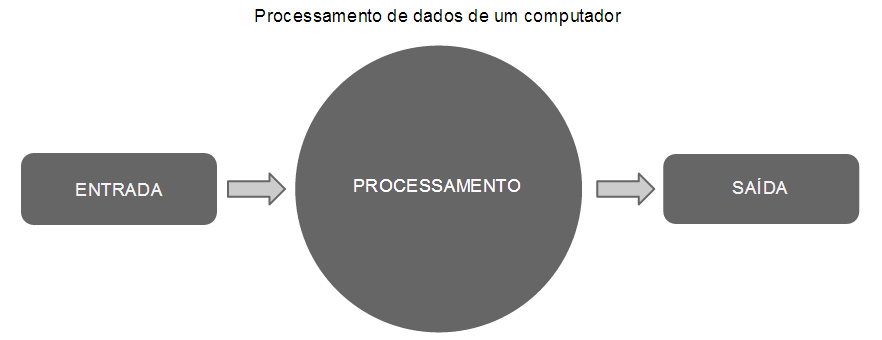
\includegraphics{images/processamento-dados-computador.png}

\subsection{Os Sistemas de Informação e o Mundo dos Negócios}\label{os-sistemas-de-informauxe7uxe3o-e-o-mundo-dos-neguxf3cios}

No mundo dos negócios as demandas (ou problemas) podem ser agrupados em 3 categorias:

\begin{itemize}
\item
  organização;
\item
  tecnologia;
\item
  pessoas;
\end{itemize}

Segundo \emph{Kenneth C. LAUDON, Jane P. LAUDON,} solucionar probelmas será sempre um processo contínuo de 4 passos:

\begin{enumerate}
\def\labelenumi{\arabic{enumi}.}
\item
  Identificar {[}do problema{]};
\item
  Receber as propostas para Solução {[}do problema{]};
\item
  Avaliar as propostas e escolher a Solução {[}do problema{]};
\item
  Implantar a SOLUÇÂO escolhida {[}para resolver o problema{]};
\end{enumerate}

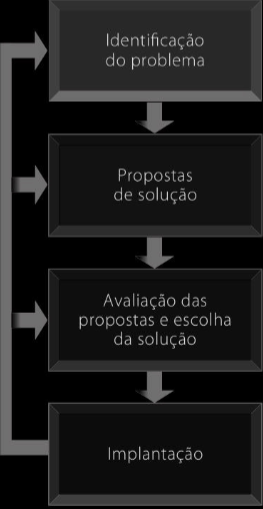
\includegraphics{images/clipboard-3657052893.png}

\section{Os diferentes Tipos de Sistemas de Informação}\label{os-diferentes-tipos-de-sistemas-de-informauxe7uxe3o}

\section{Sistemas de Informação e Vantagem Competitiva}\label{sistemas-de-informauxe7uxe3o-e-vantagem-competitiva}

\chapter{INFRAESTRUTURA DE TIC}\label{infraestrutura-de-tic}

\section{Hardware e Software}\label{hardware-e-software}

\section{Fundamentos da Inteligência de Negócios: Gestão da Informação e Banco de Dados}\label{fundamentos-da-inteliguxeancia-de-neguxf3cios-gestuxe3o-da-informauxe7uxe3o-e-banco-de-dados}

\section{Telecomunicações, Internet e Rede sem Fio}\label{telecomunicauxe7uxf5es-internet-e-rede-sem-fio}

\section{Segurança em Sistemas de Informação}\label{seguranuxe7a-em-sistemas-de-informauxe7uxe3o}

\chapter{SISTEMAS DE INFORMAÇÃO E FUNCIONALIDADES}\label{sistemas-de-informauxe7uxe3o-e-funcionalidades}

\section{Sistemas Integrados de Gestão}\label{sistemas-integrados-de-gestuxe3o}

\section{Comércio Eletrônico}\label{comuxe9rcio-eletruxf4nico}

\chapter{Tomada de Decisão de Gestão do Conhecimento: Business Inteligence}\label{tomada-de-decisuxe3o-de-gestuxe3o-do-conhecimento-business-inteligence}

\section{Ferramentas de B.I. e conceito de DashBoard}\label{ferramentas-de-b.i.-e-conceito-de-dashboard}

\subsection{PowerBI}\label{powerbi}

\section{Bancos de Dados OLTP e OLAP}\label{bancos-de-dados-oltp-e-olap}

\chapter{TECNOLOGIAS EMERGENTES E INOVAÇÃO EM TIC}\label{tecnologias-emergentes-e-inovauxe7uxe3o-em-tic}

\section{VIRTUALIZAÇÃO E CONTINENTIZAÇÃO}\label{virtualizauxe7uxe3o-e-continentizauxe7uxe3o}

\section{BIG DATA}\label{big-data}

\section{ASSISTENTES INTELIGENTES}\label{assistentes-inteligentes}

\chapter{GESTÃO DO CONHECIMENTO EM TIC}\label{gestuxe3o-do-conhecimento-em-tic}

\section{Conceitos e Práticas de Gestão do Conhecimento}\label{conceitos-e-pruxe1ticas-de-gestuxe3o-do-conhecimento}

\section{Implementação e Desafios da Gestão do Conhecimento}\label{implementauxe7uxe3o-e-desafios-da-gestuxe3o-do-conhecimento}

\chapter{APLICATIVOS DE PRODUTIVIDADE E ESCRITÓRIO I}\label{aplicativos-de-produtividade-e-escrituxf3rio-i}

\section{Planilhas Eletrônicas}\label{planilhas-eletruxf4nicas}

\section{Processadores de Texto}\label{processadores-de-texto}

\chapter{APLICATIVOS DE PRODUTIVIDADE E ESCRITÓRIO II}\label{aplicativos-de-produtividade-e-escrituxf3rio-ii}

\section{Ferramentas de Apresentação}\label{ferramentas-de-apresentauxe7uxe3o}

\section{Tecnologias de Comunicação e Colaboração}\label{tecnologias-de-comunicauxe7uxe3o-e-colaborauxe7uxe3o}

  \bibliography{book.bib,packages.bib}

\end{document}
